\documentclass[12p,a4paper]{article}
\usepackage[utf8]{inputenc}
\usepackage[T1]{fontenc,url}
\usepackage{multicol}
\usepackage{multirow}
\usepackage{parskip}
\usepackage{lmodern}
\usepackage{microtype}
\usepackage{verbatim}
\usepackage{amsmath, amssymb}
\usepackage{tikz}
\usepackage{physics}
\usepackage{mathtools}
\usepackage{algorithm}
\usepackage{algpseudocode}
\usepackage{listings}
\usepackage{enumerate}
\usepackage{graphicx}
\usepackage{float}
\usepackage{hyperref}
\usepackage{tabularx}
\usepackage{siunitx}
\usepackage{fancyvrb}
\usepackage[makeroom]{cancel}
\usepackage[margin=2cm]{geometry}
\renewcommand{\baselinestretch}{1}
\renewcommand{\exp}{e^}
\renewcommand{\b}{\boldsymbol}
\newcommand{\h}{\hat}
\newcommand{\m}{\mathbb}
\renewcommand{\d}{\mathrm{d}}
\newcommand{\half}{\frac{1}{2}}
\setlength\parindent{0pt}


\begin{document}
\title{MEK3230 -- Oblig 2}
\author{
    \begin{tabular}{r l}
        Jonas Gahr Sturtzel Lunde & (\texttt{jonassl})
    \end{tabular}}
\maketitle
\section{Fluidmekanisk labforsøk}
Levert separat til Jean.


\section{Korte oppgaver}
\subsection{}\label{sec:2.1}
Bølgene vi observerer er etter all sannsynlighet dypvannsbølger, ettersom bølgelengden og høyden er betydelig kortere enn dypet på vannet. Fasehastigheten til disse bølgene er altså $c=\SI{1}{m/s}$. Vi velger å se bort ifra kapilærbøger.\footnote{I appendiks A \ref{sec:appendiks_A} vises det at kapilærbølgene ikke ville nådd den andre siden av dammen først, selv om de var synlige.}

Det vil være bølgepakkene av dypvannsbølgene som når kanten av dammen først. Enkeltbølgene som har fasehastigheten forsvinner når de når bølgefronten, og vi kan derfor ikke bruke denne hastigheten til å studere når bølgene når kanten. Vi vet at gruppehastigheten til dypvannsbølger er gitt som
\begin{align*}
    c_g = \half c = \SI{0.5}{m/s}
\end{align*}
Dette betyr at de første bølgene vil bruke en tid
\begin{align*}
    T = \frac{\SI{10}{m}}{\SI{0.5}{m/s}} = \SI{20}{s}
\end{align*}
på å nå kanten.


\subsection{}
Inkompressibilitet er en tilnærming brukt når hastigheter i fluidet er godt under lydhastigheten i fluidet (lavt Mach tall). Man kan da gjøre antagelsen om at trykkendringer i fluidet brer seg instantant over hele systemet, som i praksis betyr at lydhastigheten er uendelig. Dette strider imot både en rekke fysiske lover, og vår oppfatning av naturen, som at lyden fra et lynnedslag kommer etter lyset. Selve definisjonen av lydhastighet blir meningsløs ved en konstant tetthet:
\begin{align*}
    c = \sqrt{\frac{\partial P}{\partial \rho}}
\end{align*}

Hvis vi betrakter et fluid med ekstremt lav kompressibilitet vil lydhastigheten kunne komme vilkårlig nære lyshastigheten, slik at lyden og lyset fra en hendelse omtrent oppfattes samtidig. Lydhastigheten vil selvsagt fortsatt aldri kunne overgå lyshastigheten, ettersom all informasjonsoverføring over lyshastighet er forbudt.


\subsubsection{}
Vi antar at parameterene som kan påvirke motstandkraften på kulen er dens radius $R$, dens synkehastighet $U$ og væskens viskositet $\mu$. Setter vi sammen disse parameterene til en dimensjonsløs gruppe, har vi bare én naturlig måte å gjøre dette på.
\begin{align*}
\Pi = \frac{F_D}{U R \mu}
\end{align*}
Løser vi dette for motstandskraften, får vi proporsjonaliteten
\begin{align*}
    F_D \propto U R \mu
\end{align*}


\subsubsection{}
Fordi vi har krypstrøm ($Re=0$), vil
\begin{align*}
    F_1 = F_2
\end{align*}

Dette er fordi krypstrøm er reversibelt. Hvis du forestiller deg at du drar legemet en distanse gjennom det viskøse fluidet, for deretter å reversere hastigheten og dra det tilbake til utgangsposisjonen, vil alle fluid-partiklene følge samme partikkelbane baklengs på veien tilbake, grunnet reversibiliteten. Arbeidet gjort på fluidet over denne distansen må altså være identisk i begge retninger, og kraften må da være lik.


\section{Lange oppgaver}
\subsection{}
\subsubsection{}
Vi tar utgangspunkt i Navier Stokes.
\begin{align*}
    \frac{Dh}{Dt} = -\frac{1}{\rho}\frac{\partial}{\partial z} P + \nu \nabla^2 w - g
\end{align*}
For at hydrostatisk trykk skal gi mening, antar vi at fluidet har nådd en tilnærmet likevekt, og vi stryker alle hastighetsledd.
\begin{align*}
    0 = -\frac{1}{\rho}\frac{\partial}{\partial z} P - g \\
    P = - \rho g z + c_1
\end{align*}
Vi løser for $c_1$ ved å benytte at trykket ved $z=H_n$ er $P(z=H_n) = P_0$. Dette betyr at trykket ved fluidets overflate, $z=h$ er $P(z=h) = P_0 + (\rho - \Delta\rho)g(H_d - h)$. Setter vi dette lik uttrykket vårt for $P$, får vi
\begin{align*}
    P(z=h) = - \rho g z + c_1 = P_0 + \qty(\rho - \Delta\rho)g(H_d - h) \\
    \Rightarrow \quad c_1 = \rho g h + P_0 + \qty(\rho - \Delta\rho)(H_d - h)\\
    = P_0 + \rho g h + \rho g H_d - \Delta\rho g H_d - \rho g h + \Delta\rho g h\\
    = P_0 + \rho g H_d - \Delta\rho g H_d + \Delta\rho g h
\end{align*}
som gir det hydrostatiske trykket
\begin{align}\label{eqn:hydrostatic}
    P(z) = -\rho g z + P_0 + \rho g H_d - \Delta\rho g H_d + \Delta\rho g h
\end{align}


\subsubsection{}
Vi starter med Navier Stokes.
\begin{align*}
    \frac{\partial\b u}{\partial t} + \b u \cdot \nabla \b u = -\frac{1}{\rho}\nabla P + \nu \nabla^2\b u - \b g
\end{align*}
Vi antar stasjonær strømning, og krypstrøm, slik at det tidsderiverte leddet og treghetsleddet faller.
\begin{align*}
    0 = -\frac{1}{\rho} \qty(\frac{\partial}{\partial x}P,\ \frac{\partial}{\partial y}P,\ \frac{\partial}{\partial z}P) + \nu \qty(\frac{\partial^2}{\partial x^2}\b u + \frac{\partial^2}{\partial y^2}\b u + \frac{\partial^2}{\partial z^2}\b u) \\
    \frac{1}{\rho} \qty(\frac{\partial}{\partial x}P,\ \frac{\partial}{\partial y}P,\ \frac{\partial}{\partial z}P) = \nu \qty(\frac{\partial^2}{\partial z^2}\b (u,\, v,\ w))
\end{align*}
Ettersom vi ser på tilfellet $h_0/l \ll 1$, kan vi anta at det z-dervierte leddet dominerer.
\begin{align*}
    \frac{\partial}{\partial x}P = \mu \frac{\partial^2}{\partial z^2} u \\
    \frac{\partial}{\partial y}P = \mu \frac{\partial^2}{\partial z^2} v \\
    \frac{\partial}{\partial z}P = \mu \frac{\partial^2}{\partial z^2} w
\end{align*}



\subsubsection{}
\paragraph{Grensebetingelser.}
Vi introduserer først grensebetingelsene for fluidet.
%Siden vi jobber med viskøs teori, har vi "no-slip", altså at det ikke foregår noen bevegelse av fluidet i grensesjiktet mellom fluidet og den solide flaten.
Fluidet kan ikke ha noen hastighet i z-retning i overflatesjiktet til den solide flaten, altså ved $z=0$. "No-penetration" grensebetingelsen gir
\begin{align}\label{GB:no_pen}
    w(z=0) = 0
\end{align}
Vi har også den kinematiske grensebetingelsen, som sier at fluidpartikkelens z-hastighet ved fluidets overflate må følge overflatens bevegelse:
\begin{align}\label{GB:kin}
    w(z=h) = \frac{\partial h}{\partial t} + u \frac{\partial h}{\partial x}
\end{align}
Til slutt har vi betingelsen om ingen skjærspenning ved overflaten
\begin{align}\label{GB:sheer_stress}
    \mu\frac{\partial u(z=h)}{\partial z} = 0
\end{align}


\paragraph{Kontinuitetsligningen.}
Vi gjør først en liten de-tour for å finne et resultat vi trenger senere. Vi tar utgangspunkt i kontinuitetsligningen,
\begin{align*}
    \nabla \cdot \b u = 0
\end{align*}
og integrerer hver side over sirupens høyde, fra $0$ til $h(x,t)$:
\begin{align*}
    \int\limits_0^{h(x,t)}\qty(\frac{\partial u}{\partial x} + \frac{\partial w}{\partial z})\d z = 0 \\
    \int\limits_0^{h(x,t)}\frac{\partial u}{\partial x}\d z + \int\limits_0^{h(x,t)}\partial w = 0
\end{align*}
Ved å benytte Leibniz' integralteorem, får vi at venstresiden blir
\begin{align*}
    \frac{\partial}{\partial x}\int\limits_0^{h(x,t)}u\, \d z - u\frac{\partial h}{\partial x} + w\Big|_0^h
\end{align*}
Ved insetting av \ref{GB:no_pen} og \ref{GB:kin} får vi
\begin{align*}
    = \frac{\partial}{\partial x}\int\limits_0^{h(x,t)}u\, \d z - u\frac{\partial h}{\partial x} + \frac{\partial h}{\partial t} + u \frac{\partial h}{\partial x}
\end{align*}
\begin{align}\label{eqn:int_u}
    \frac{\partial}{\partial x}\int\limits_0^{h(x,t)}u\, \d z + \frac{\partial h}{\partial t} = 0
\end{align}



\paragraph{Stokes ligning.}
Vi tar utgangspunkt i ligningen for krypstrøm i z-retning:
\begin{align*}
    \nabla P = \mu\nabla^2 \b u
\end{align*}
\begin{align*}
    \frac{\partial P}{\partial x} = \mu\frac{\partial^2 u}{\partial z^2} \\
    \frac{\partial P}{\partial x}z + c_1 = \mu\frac{\partial u}{\partial z}
\end{align*}
For å løse for $c_1$ ser vi på ligningen ved overflaten, $z=h$, og benytter oss av grensebetingelsen om skjærstress, \ref{GB:sheer_stress}:
\begin{align*}
    \frac{\partial P}{\partial x}h + c_1 = 0
    \quad \Rightarrow \quad c_1 = -\frac{\partial P}{\partial x}h
\end{align*}
som gir ligningen
\begin{align*}
    \frac{\partial P}{\partial x}z -\frac{\partial P}{\partial x}h = \mu\frac{\partial u}{\partial z}
\end{align*}
som vi løser for $u$ ved å integrere med hensyn på z.
\begin{align*}
    u = \frac{1}{\mu}\frac{\partial P}{\partial x}\qty[\half z^2 - hz]
\end{align*}
Integrerer vi dette igjen med hensyn på z, over sirupens høyde ($0$ til $h(x,t)$) får vi
\begin{align*}
    \int\limits_0^{h(x,t)}u\, \d z = \frac{1}{\mu} \frac{\partial P}{\partial z}\qty[\frac{1}{6}z^3 - \half z^3] = -\frac{1}{3\mu} \frac{\partial P}{\partial z} h^3
\end{align*}
Setter vi dette uttrykket inn i ligning \ref{eqn:int_u} får vi
\begin{align}\label{eqn:hP}
    \frac{\partial h}{\partial t} - \frac{\partial}{\partial x}\qty[\frac{h^3}{3\mu}\frac{\partial P}{\partial x}] = 0
\end{align}
Setter vi inn for det hydrostatiske trykket definert i \ref{eqn:hydrostatic}, får vi, ettersom bare $\Delta\rho g h$ leddet inneholder noe deriverbart med $x$:
\begin{align}\label{eqn:h}
    \frac{\partial h}{\partial t} - \frac{\partial}{\partial x}\qty[\frac{gh^3 \Delta\rho}{3\mu}\frac{\partial h}{\partial x}h^3] = 0
\end{align}


\subsubsection{}
Ved insetting av de oppgitte skaleringsfaktorene blir ligning \ref{eqn:h} til
\begin{align}\label{eqn:HT}
    \frac{\partial H}{\partial T}\frac{g\Delta\rho h_0^4}{3L^2\mu} - \frac{\partial}{\partial X}\frac{1}{L}\qty[\frac{gH^3h_0^3\Delta\rho}{3\mu}\frac{\partial H}{\partial X}\frac{h_0}{L}] = 0 \\
    \frac{\partial H}{\partial T} - \frac{\partial}{\partial X}\qty[H^3\frac{\partial H}{\partial X}] = 0
\end{align}

Vi skal nå anta at høyden og bredden på sirupen kan skrives som en power law av tiden, på formen
\begin{align*}
    X_n \propto T^{\alpha} \\
    H_n \propto T^{\beta}
\end{align*}
Vi infører en variabel for sirupens areal i $xz$-planet, $q = X_nH_n$, slik at \begin{align*}
    H_n = \frac{q}{X_n} \propto \frac{1}{X_n}
\end{align*}
Hvis vi kun studerer proporsjonalitet av karakteristiske størrelser i ligning \ref{eqn:HT}, får vi at
\begin{align*}
    \frac{H_n}{T} \propto \frac{1}{X_n}\qty[H_n^3\frac{H_n}{X_n}] \\
    \frac{1}{X_nT} \propto \frac{1}{X_n}\qty[\frac{1}{X_n^3}\frac{1}{X_n^2}]\\
\end{align*}
som gir proporsjonaliteten
\begin{align*}
    X_n \propto T^{1/5}
\end{align*}
Ved insetting av $H_n \propto \frac{1}{X_n}$ får vi også at
\begin{align*}
    H_n \propto T^{-1/5}
\end{align*}



\subsubsection{}
Programmet ligger vedlagt i appendiks B \ref{sec:appendiks_B}. For å få programmet til å kjøre, legg ved en
\begin{verbatim}
    np.save("data.npy", H)
\end{verbatim}
i det utdelte programmet.\footnote{Jeg ble lei av å vente 20 sekunder hver gang jeg skulle gjøre en liten endring i programmet, så jeg skrev dataene til en binærfil, og henter de ut i programmet mitt.} Nedenfor ser vi høyden og bredden av sirupen over tid, plottet mot stigningstallet de skal være proporsjonale med. Vi ser at begge grafene har samme stigningtall som vi analytisk forventet. (grafene er selvsagt bare proporsjonale, og ikke identiske, ettersom vi bare har regnet ut power-law faktoren.)

\begin{figure}[H]
    \centering
    \includegraphics[width=0.8\textwidth]{{X_n.pdf}}
    \caption{Bredde - $X_n(T)$}
    \label{}
\end{figure}

\begin{figure}[H]
    \centering
    \includegraphics[width=0.8\textwidth]{{H_n.pdf}}
    \caption{Høyde - $H_n(T)$}
    \label{}
\end{figure}


\subsubsection{}
Under ser vi et skalert plott av alle løsnigene. Vi ser at de for alle praktiske formål er selv-similiare. Det virker å være en liten forskyvning mellom hvert av plottene. Dette kan enten være min feil, eller en begrensning av vår numeriske løsningsmetode.
\begin{figure}[H]
    \centering
    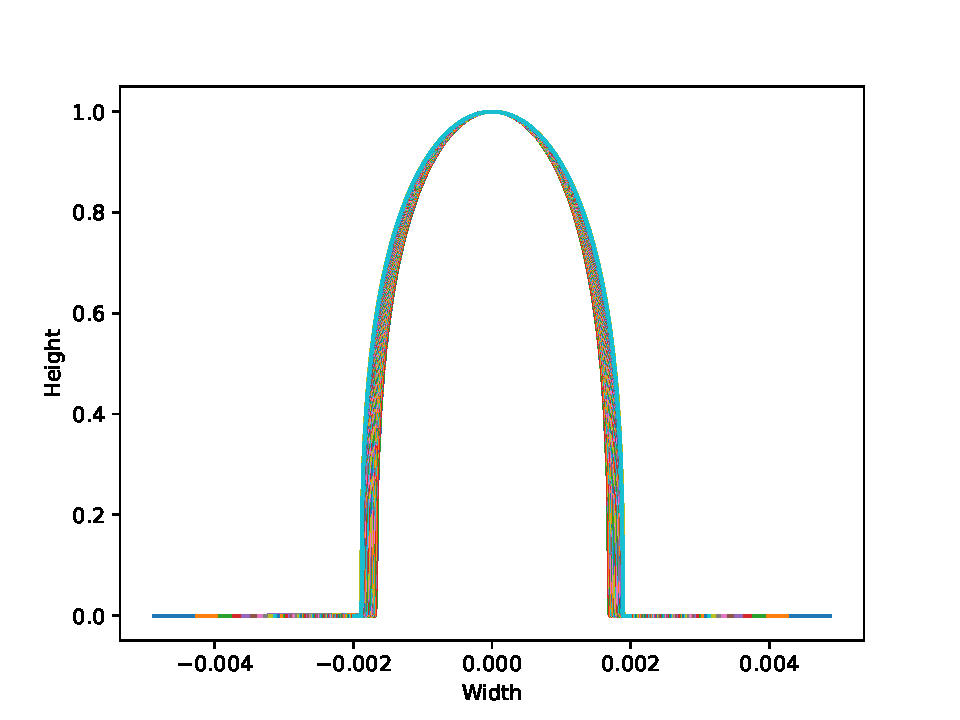
\includegraphics[width=0.8\textwidth]{similiarity.pdf}
    \caption{Similaritet av løsningene}
    \label{}
\end{figure}

\subsubsection{}
\paragraph{Overflatespenning og Bond tallet.}
Vi tar igjen utgangspunkt i ligning \ref{eqn:hP}, men denne gangen inkluderer vi overflatespenningen i trykkleddet, slik at vi setter trykket som $p* = -p -\gamma\frac{\partial^2 h}{\partial x^2}$, der $p$ er det gamle trykket. Vi får
\begin{align*}
    \frac{\partial h}{\partial t} - \frac{\partial}{\partial x}\qty[\frac{h^3}{3\mu}\frac{\partial(-p-\gamma\frac{\partial^2 h}{\partial x^2})}{\partial x}] =
    \frac{\partial h}{\partial t} + \frac{\partial}{\partial x}\qty[\frac{h^3}{3\mu}\qty(\frac{\partial p}{\partial x} + \frac{\partial \gamma\frac{\partial^2 h}{\partial x^2}}{\partial x})] \\
    = \frac{\partial h}{\partial t} + \frac{\partial}{\partial x}\qty[\frac{gh^3\Delta\rho}{3\mu}\frac{\partial h}{\partial x} + \frac {\gamma h^3}{3\mu}\frac{\partial^3 h}{\partial x^3}]
\end{align*}
Skalering med de oppgitte verdiene gir
\begin{align*}
    \frac{\partial H}{\partial T}\frac{g\Delta\rho h_0^4}{3L\mu} + \frac{\partial}{\partial X}\frac{1}{L}\qty[\frac{gH^3h_0^3\Delta\rho}{3\mu}\frac{\partial H}{\partial X}\frac{h_0}{L} + \frac{\gamma H^3h_0^3}{3\mu}\frac{\partial^3 H}{\partial X^3}\frac{h_0}{L^3}] \\
    = \frac{\partial H}{\partial T} + \frac{\partial}{\partial X}\qty[H^3\qty(\frac{\partial H}{\partial X} + \frac{\gamma}{\Delta\rho g L^2} \frac{\partial^3 H}{\partial X^3})]
\end{align*}
\begin{align}\label{eqn:H_Bo}
        \frac{\partial H}{\partial T} + \frac{\partial}{\partial X}\qty[H^3\qty(\frac{\partial H}{\partial X} + \frac{1}{\mathrm{Bo}} \frac{\partial^3 H}{\partial X^3})] = 0
\end{align}
som gjør Bond-tallet til
\begin{align*}
    \mathrm{Bo} = \frac{\Delta\rho g L^2}{\gamma}
\end{align*}

\paragraph{Linearisering.}
Vi introduserer lineariseringen av $H$ som $H = H_0 + \epsilon \h H(X,T)$ der $H_0$ er en konstant med hensyn på tid og rom. Vi setter inn lineariseringen i \ref{eqn:H_Bo}, og tar hensyn til at både tidlige og romlige derivasjoner av $H_0$ er 0. Vi stryker også det siste leddet, som får en faktor $\epsilon^3$
\begin{align*}
    \epsilon\frac{\partial \h H}{\partial T} + \frac{\partial}{\partial X}\qty[(H_0 + \epsilon \h H)^3\qty(\epsilon\frac{\partial \h H}{\partial X} + \epsilon\frac{\partial^3 \h H}{\partial X^3})] = 0
\end{align*}
Skriver vi ut parantesen, og stryker alle ledd $\leq \mathrm{O}(\epsilon^2)$, får vi
\begin{align*}
    \epsilon\frac{\partial \h H}{\partial T} + \frac{\partial}{\partial X}\qty[H_0^3 \epsilon \frac{\partial \h H}{\partial X} + H_0^3 \epsilon\frac{\partial^3 \h H}{\partial X^3})] = 0
\end{align*}
\begin{align}\label{eqn:lin_H}
    \frac{\partial \h H}{\partial T} + H_0^3\frac{\partial^2 \h H}{\partial X^2} + H_0^3\frac{\partial^4 \h H}{\partial X^4} = 0
\end{align}


\subsubsection{}
Ved insetting av pertubasjonen $\h H(X,T) = \exp{i(kX - \omega T)}$ i den lineariserte ligningen \ref{eqn:lin_H}, får vi
\begin{align*}
    \frac{\partial \exp{i(kX - \omega T)}}{\partial T} + H_0^3\frac{\partial^2 \exp{i(kX - \omega T)}}{\partial X^2} + H_0^3\frac{\partial^4 \exp{i(kX - \omega T)}}{\partial X^4} = 0 \\
    \\
    -i\omega \exp{i(kX - \omega T)} - H_0^3 k^2 \exp{i(kX - \omega T)} + H_0^3 k^4\exp{i(kX - \omega T)} = 0
\end{align*}
som gir oss dispersjonsrelasjonen
\begin{align}
    \omega(k) = iH_0^3k^2\qty(1 - k^2)
\end{align}
Setter vi dette inn i pertubasjonen, får vi
\begin{align*}
    \h H(X,T) = \exp{i(kX - iH_0^3k^2\qty(1 - k^2) T)} = \exp{H_0^3k^2\qty(1 - k^2)T}\exp{ikX} = \exp{\sigma_R T}\exp{ikX}
\end{align*}
Fluidet blir over tid ustabilt for $\sigma_R > 0$ og stabilt for $\sigma_R < 0$, ettersom dette leddet bestemmer om den reelle eksponenten går mot 0 eller uendelig. Dette betyr at vi må kreve at
\begin{align*}
    H_0^3k^2\qty(1 - k^2) \leq 1 \\
    0 \leq H_0 \leq 2^{2/3}
\end{align*}
for at fluidet skal holdes stabilt. Jeg er litt skeptisk til at dette er korrekt, spesielt i og med at $k$ har forsvunnet...




\subsection{}
\subsubsection{}
Vi kan bruke et hastighetspotensial for å beskrive en strømning dersom hastighetsfeltet er virvelfritt. Dette vil si at $\nabla \times \b u(t) = 0$ for alle $t$. Vi kan forenkle dette kravet ved å isteden kreve at hastighetsfeltet er virvelfritt på ett virkårlig tidspunkt $t_0$ (gjerne $t_0=0$):
\begin{align*}
    \nabla \times \b u(t_0) = 0
\end{align*}
og samtidig kreve at strømningen er friksjonsfri (ikke-viskøs, $\mathrm{Re} = \infty$). Det kan ikke oppstå virvling i et friksjonsfritt felt der det på et tidspunkt ikke er virvling.


\subsubsection{}
Vi kan kreve at det ikke er noen vertikal hastighet ved veggene (no-penetration), ettersom dette ville innebære at væske går gjennom veggene.
\begin{align}
    w_1(z = H) = \frac{\partial \psi_1}{\partial z} = 0 \\
    w_2(z = -H) = \frac{\partial \psi_2}{\partial z} = 0
\end{align}

Ettersom fluidene ligger inntil hverandre kan vi kreve at hastighetspotensialet er likt ved overflaten.
\begin{align}
    \psi_1(z=0) = \psi_2(z=0)
\end{align}

Vi har også den kinematiske grenseflatebetingelsen
\begin{align}
    \frac{\partial \eta}{\partial t} = \frac{\partial \psi}{\partial z}
\end{align}


\subsubsection{}
Vi har de to hastighetspotensialene som
\begin{align*}
    \psi_1 = A\cosh(B)\cos(C) \\
    \psi_2 = D\cosh(E)\cos(F)
\end{align*}

Vi antar å kunne beskrive overflaten på den vanlige bølgeformen
\begin{align*}
    \eta(x,t) = a\sin(kx - \omega t)
\end{align*}

Her rakk jeg dessverre ikke mer :)

\section{Appendiks A - Kapilærbølger fra stein}\label{sec:appendiks_A}
I \ref{sec:2.1} antok vi at bare gravitasjonsbølgene var synlige når vi slapp steinen i dammen. Vi skal nå anta at bølgelengden er tilstrekkelig kort til at kapilære bølger ikke er helt neglisjerbare. De første bølgene som når kanten kan da være kapilærbølger, hvis de har tilstrekkelig hastighet. Gruppehastigheten til kapilærbølger er gitt som
\begin{align}\label{eqn:cg}
    c_g = \frac{3}{2}\sqrt{\frac{\gamma k}{\rho}}
\end{align}

Det vil selvsagt også fortsatt oppstå dypvannsbølger. Dypvannnsbølger har en bølgehastighet(fasehastighet) på
\begin{align*}
    c = \sqrt{\frac{g}{k}} = 1\si{m/s}
\end{align*}
som gir at
\begin{align*}
    k = g
\end{align*}
Setter vi dette inn i \ref{eqn:cg}, sammen med tettheten ($\rho \approx \SI{1000}{kg/m^3}$) og overflatespenningen ($\gamma \approx \SI{0.072}{J/m^2}$) til vann ved 25 grader, får vi at gruppehastigheten til kapilærbølgene er
\begin{align*}
    c_g = \frac{3}{2}\sqrt{\frac{\SI{0.072}{J/m^2} \cdot \SI{9.81}{m^{-1}}}{\SI{1000}{kg/m^3}}} \approx \SI{0.04}{m/s}
\end{align*}
Dette er altså betydelig saktere enn dypvannsbølgene, og kapilærbølgene vil ikke nå den andre siden av dammen først, selv om de er synlige.


\section{Appendiks B - Kode}\label{sec:appendiks_B}
\verbatiminput{program.py}

\end{document}
